\subsection{SMO算法}

\subsubsection{坐标上升}
\begin{enumerate}
	\item 坐标上升要优化的问题可描述为:
	\begin{align}
		\max_{\alpha}W(\alpha_1, \alpha_2, \dots, \alpha_m)
	\end{align}
	我们先不管那些约束条件
	\item 坐标上升优化方法 \\ 
	Loop until convergence: \{ \\
		For i = 1, ..., m: \{ \\
			$\alpha_i := \arg \max_{\hat{\alpha_i}}W(\alpha_1, \dots, \alpha_{i-1}, \alpha_i, \alpha_{i+1}, \dots, \alpha_m)$ \\
		\} \\
	\} 
	\item 在最内层循环中,我们固定住除$\alpha_i$外的所有$\alpha$,令$i=1 \to m$,通过这种方式一直优化,直到收敛
	\item 坐标上升算法示意图
	\begin{figure}[htbp]
		\centering
		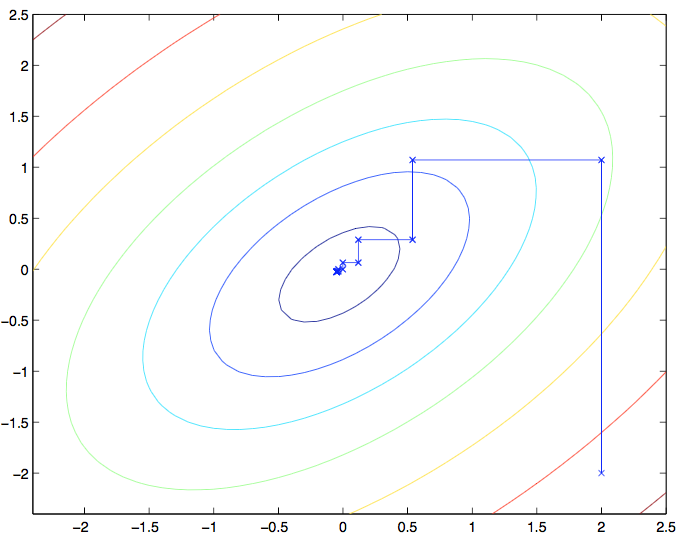
\includegraphics[scale=0.8]{./images/坐标上升}
		\caption{坐标上升示意图}
	\end{figure}
\end{enumerate}


\subsubsection{SMO}
在我们的SVM中,如果还是像前面的坐标上升算法那样固定住除$\alpha_j$以外的所有$\alpha$,那么,因为约束条件的存在,$\alpha_j$也被约束条件固定下来了,所以,我们就让两个$\alpha$可变,这就有了SMO。\\
详略,暂时不想写,参考资料:\url{http://www.cnblogs.com/jerrylead/archive/2011/03/18/1988419.html}
